\documentclass{article}
\usepackage{fullpage}
\usepackage{indentfirst}
\usepackage{amsmath}
\usepackage{amsfonts}
\usepackage{array}
\usepackage{tipa}
\usepackage{tikz}
\usepackage{tikz-qtree}
\usetikzlibrary{matrix, arrows, automata}
\usepackage{gb4e}
\noautomath
\newcommand{\Y}{$\checkmark$}
\newcommand{\N}{\ding{55}}
\newcommand{\R}{$\Rightarrow$}
\newcommand\myeq{\mathrel{\stackrel{\makebox[0pt]{\mbox{\normalfont\tiny def}}}{=}}}
\title{Multi-syllable Models}
\author{Chris Oakden}
\begin{document}
\maketitle
The goal here is to make a general model for both Bao and Yip models for polysyllabic forms, like below.
\begin{center}
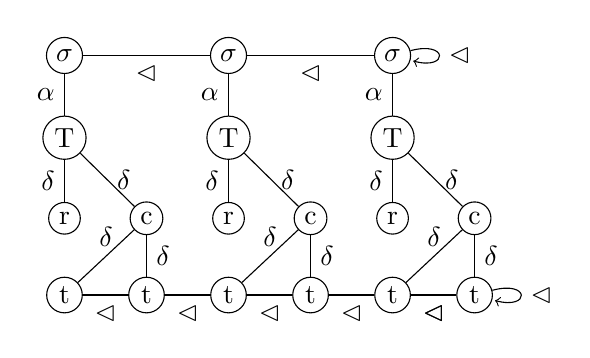
\begin{tikzpicture} [baseline = (x.base)]
\matrix (m) [matrix of nodes, column sep = 1.5em, row sep = 1.5em]{
\node[draw,circle, inner sep =2pt](x){$\sigma$}; & & \node[draw,circle, inner sep =2pt](x2){$\sigma$}; & & \node[draw,circle, inner sep =2pt](x3){$\sigma$};  \\
\node[draw,circle, inner sep =2pt](y){T}; & & \node[draw,circle, inner sep =2pt](y2){T}; & & \node[draw,circle, inner sep =2pt](y3){T};  \\
\node[draw,circle, inner sep =2pt](z){r}; & \node[draw,circle, inner sep =2pt](v){c}; & \node[draw,circle, inner sep =2pt](z2){r}; & \node[draw,circle, inner sep =2pt](v2){c}; & \node[draw,circle, inner sep =2pt](z3){r}; & \node[draw,circle, inner sep =2pt](v3){c};\\
\node[draw,circle, inner sep =2pt](q){t}; & \node[draw,circle, inner sep =2pt](s){t}; & \node[draw,circle, inner sep =2pt](q2){t}; & \node[draw,circle, inner sep =2pt](s2){t}; & \node[draw,circle, inner sep =2pt](q3){t}; & \node[draw,circle, inner sep =2pt](s3){t}; \\
};
\draw (x) -- (y) node[left, pos=.5]{$\alpha$};
\draw (z) -- (y) node[left, pos=.5]{$\delta$};
\draw (v) -- (y) node[right, pos=.5]{$\delta$};
\draw (q) -- (v) node[above, pos=.5]{$\delta$};
\draw (s) -- (v) node[right, pos=.5]{$\delta$};
\draw (q) -- (s) node[below, pos=.5]{$\vartriangleleft$};
\draw (x2) -- (y2) node[left, pos=.5]{$\alpha$};
\draw (z2) -- (y2) node[left, pos=.5]{$\delta$};
\draw (v2) -- (y2) node[right, pos=.5]{$\delta$};
\draw (q2) -- (v2) node[above, pos=.5]{$\delta$};
\draw (s2) -- (v2) node[right, pos=.5]{$\delta$};
\draw (q2) -- (s2) node[below, pos=.5]{$\vartriangleleft$};
\draw (x3) -- (y3) node[left, pos=.5]{$\alpha$};
\draw (z3) -- (y3) node[left, pos=.5]{$\delta$};
\draw (v3) -- (y3) node[right, pos=.5]{$\delta$};
\draw (q3) -- (v3) node[above, pos=.5]{$\delta$};
\draw (s3) -- (v3) node[right, pos=.5]{$\delta$};
\draw (q3) -- (s3) node[below, pos=.5]{$\vartriangleleft$};
\draw (q3) -- (s3) node[below, pos=.5]{$\vartriangleleft$};
\draw (x) -- (x2) node[below, pos=.5]{$\vartriangleleft$};
\draw (x2) -- (x3) node[below, pos=.5]{$\vartriangleleft$};
\draw (s) -- (q2) node[below, pos=.5]{$\vartriangleleft$};
\draw (s2) -- (q3) node[below, pos=.5]{$\vartriangleleft$};
\path (x3) edge [loop right, align = center] node{$\vartriangleleft$} (x3);
\path (s3) edge [loop right, align = center] node{$\vartriangleleft$} (s3);
\end{tikzpicture}
\hspace{1.2cm}
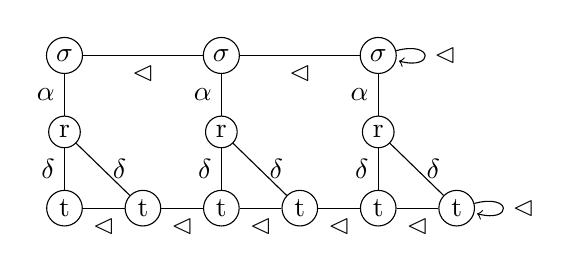
\begin{tikzpicture} [baseline = (x.base)]
\matrix (m) [matrix of nodes, column sep = 1.5em, row sep = 1.5em]{
\node[draw,circle, inner sep =2pt](x){$\sigma$}; & & \node[draw,circle, inner sep =2pt](x2){$\sigma$}; & & \node[draw,circle, inner sep =2pt](x3){$\sigma$};  \\
\node[draw,circle, inner sep =2pt](y){r}; & & \node[draw,circle, inner sep =2pt](y2){r}; & & \node[draw,circle, inner sep =2pt](y3){r};  \\
\node[draw,circle, inner sep =2pt](z){t}; & \node[draw,circle, inner sep =2pt](v){t}; & \node[draw,circle, inner sep =2pt](z2){t}; & \node[draw,circle, inner sep =2pt](v2){t}; & \node[draw,circle, inner sep =2pt](z3){t}; & \node[draw,circle, inner sep =2pt](v3){t};\\
};
\draw (x) -- (y) node[left, pos=.5]{$\alpha$};
\draw (z) -- (y) node[left, pos=.5]{$\delta$};
\draw (v) -- (y) node[right, pos=.5]{$\delta$};
\draw (x2) -- (y2) node[left, pos=.5]{$\alpha$};
\draw (z2) -- (y2) node[left, pos=.5]{$\delta$};
\draw (v2) -- (y2) node[right, pos=.5]{$\delta$};
\draw (x3) -- (y3) node[left, pos=.5]{$\alpha$};
\draw (z3) -- (y3) node[left, pos=.5]{$\delta$};
\draw (v3) -- (y3) node[right, pos=.5]{$\delta$};
\draw (x) -- (x2) node[below, pos=.5]{$\vartriangleleft$};
\draw (x2) -- (x3) node[below, pos=.5]{$\vartriangleleft$};
\draw (v) -- (z2) node[below, pos=.5]{$\vartriangleleft$};
\draw (v2) -- (z3) node[below, pos=.5]{$\vartriangleleft$};
\draw (z) -- (v) node[below, pos=.5]{$\vartriangleleft$};
\draw (z2) -- (v2) node[below, pos=.5]{$\vartriangleleft$};
\draw (z3) -- (v3) node[below, pos=.5]{$\vartriangleleft$};
\path (x3) edge [loop right, align = center] node{$\vartriangleleft$} (x3);
\path (v3) edge [loop right, align = center] node{$\vartriangleleft$} (v3);
\end{tikzpicture}
\end{center}
Several assumptions are inherent in the above figures. One is that order is only imposed on TBU (syllable) and terminal tonal nodes, and crucially not on heterosyllabic register (r), contour (c), or tonal root node (T) nodes. The other is that order is imposed on terminal tonal nodes \emph{between syllables}. Both tiers are ordered via the successor function, and order is total within each tier (s.t. the final element is its own successor). We will explore the impact of these assumptions on expanding the general model to such forms, and change these assumptions somewhat as we go. \par
Generally speaking, the only changes between the mono- and polysyllabic general models are the association, dominance, and successor functions. Unary relations do not change. Let us begin simply with a disyllabic Yip model. Recall the previous model...
\begin{equation}
\mathfrak{M}^{Y} \myeq \langle\mathfrak{D}; \mathcal{P}_{rf}, \mathcal{P}_{cf}, \mathcal{P}_{tbu}; \alpha(x), \delta(x), \mathtt{succ}(x)\rangle \\
\end{equation}
...and the general definitions of association and dominance:
\begin{equation} \label{Yipoldfunctions}
\alpha(x) = y \myeq P_{\sigma}(x) \land P_{rf}(y) \qquad \delta(x) = y \myeq P_{cf}(x) \land P_{rf}(y)
\end{equation}
Clearly, the definitions in (\ref{Yipoldfunctions}) are insufficient for a polysyllabic general model, as they predict association and dominance relations to hold \emph{between syllables}, basically creating a lattice-like pattern for functions. Consider association and dominance in a trisyllabic form given the current definitions.
\begin{center}
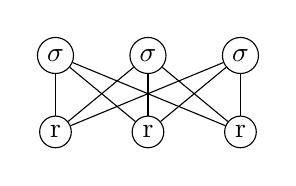
\begin{tikzpicture} [baseline = (x1.base)]
\matrix (m) [matrix of nodes, column sep = 2em, row sep = 1.5em]{
\node[draw, circle, inner sep = 2pt](x1){$\sigma$}; & \node[draw, circle, inner sep = 2pt](x2){$\sigma$}; & \node[draw, circle, inner sep = 2pt](x3){$\sigma$}; \\
\node[draw, circle, inner sep = 2pt](y1){r}; & \node[draw, circle, inner sep = 2pt](y2){r}; & \node[draw, circle, inner sep = 2pt](y3){r}; \\   
};
\draw (x1) -- (y1);
\draw (x1) -- (y2);
\draw (x1) -- (y3);
\draw (x2) -- (y1);
\draw (x2) -- (y2);
\draw (x2) -- (y3);
\draw (x3) -- (y1);
\draw (x3) -- (y2);
\draw (x3) -- (y3);
\end{tikzpicture}
\hspace{2cm}
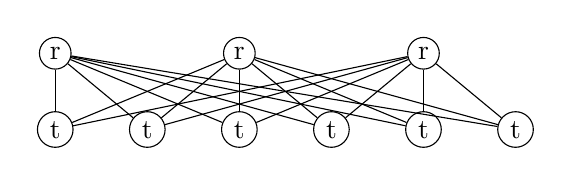
\begin{tikzpicture} [baseline = (x1.base)]
\matrix (m) [matrix of nodes, column sep = 2em, row sep = 1.5em]{
\node[draw, circle, inner sep = 2pt](x1){r}; & & \node[draw, circle, inner sep = 2pt](x2){r}; & & \node[draw, circle, inner sep = 2pt](x3){r}; \\
\node[draw, circle, inner sep = 2pt](y1){t}; & \node[draw, circle, inner sep = 2pt](y2){t}; & \node[draw, circle, inner sep = 2pt](y3){t}; & \node[draw, circle, inner sep = 2pt](y4){t}; & \node[draw, circle, inner sep = 2pt](y5){t}; & \node[draw, circle, inner sep = 2pt](y6){t}; \\   
};
\draw (x1) -- (y1);
\draw (x1) -- (y2);
\draw (x1) -- (y3);
\draw (x1) -- (y4);
\draw (x1) -- (y5);
\draw (x1) -- (y6);
\draw (x2) -- (y1);
\draw (x2) -- (y2);
\draw (x2) -- (y3);
\draw (x2) -- (y4);
\draw (x2) -- (y5);
\draw (x2) -- (y6);
\draw (x3) -- (y1);
\draw (x3) -- (y2);
\draw (x3) -- (y3);
\draw (x3) -- (y4);
\draw (x3) -- (y5);
\draw (x3) -- (y6);
\end{tikzpicture}
\end{center}
We must restrict dominance and association to tautosyllabic nodes. But how? \par
A promising approach to achieving such restriction is to make use of order. In fact, there is only order available to us to disambiguate syllable nodes and ensure that association and domination stay within a syllable (while still keeping the definitions QF). This entails defining a function such that the same function applied to the successor of its domain will yield the successor of the codomain. In other words, $f(x) = y \land f(succ(x)) = succ(y)$. Since only the syllabic and terminal tonal tiers are ordered, it will be tricky to set up the necessary reference points. We refer to the register node and its successor via its sub, the terminal tonal nodes (which have an order). We therefore append the definition of $\alpha(x)$:
\begin{equation}
\alpha(x) = y \myeq P_{\sigma}(x)\,\land\,\delta(P_{cf}(y))\,\land[\alpha(\delta(succ(y)))=succ(x)]
\end{equation}
The above definition is recursive in a sense. The base case is a syllable (the TBU) and the `dominator of a terminal node' (=register). The recursive part of the definition states that the successor of the syllable node is also in the same relationship with the `dominator of the successor of y' (the register node of the following syllable). \\
\begin{center}
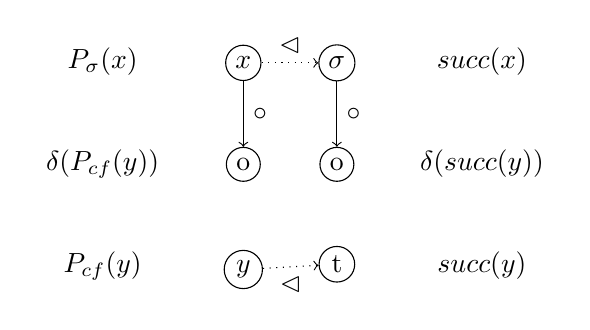
\begin{tikzpicture} [baseline = (m-1-1.base)]
\matrix (m) [matrix of nodes, column sep = 2em, row sep = 2em]{
$P_{\sigma}(x)$ & \node[draw,circle, inner sep =2pt](x1){$x$}; & \node[draw,circle, inner sep =2pt](x2){$\sigma$}; & $succ(x)$ \\
$\delta(P_{cf}(y))$ & \node[draw,circle, inner sep =2pt](y1){o}; & \node[draw,circle, inner sep =2pt](y2){o}; & $\delta(succ(y))$  \\
$P_{cf}(y)$ & \node[draw,circle, inner sep =2pt](z1){$y$}; & \node[draw,circle, inner sep =2pt](z2){t}; & $succ(y)$ \\
};
\draw [->] (x1) -- (y1) node[right, pos = .5]{$\circ$};
\draw [->] (x2) -- (y2) node[right, pos = .5]{$\circ$};
\draw [->, dotted] (x1) -- (x2) node[above, pos = .5]{$\vartriangleleft$};
\draw [->, dotted] (z1) -- (z2) node[below, pos = .5]{$\vartriangleleft$};
\end{tikzpicture}
\end{center}
At first glance, this definition is unappealing, because it requires reference to both association and dominance. This may be unavoidable, however. \par
Another option is to impose an order on the intermediate nodes across syllables (for example to define $succ(x)$ over register nodes). Recursion is also necessary, but the intuition comes through a bit more clearly.
\begin{equation}
\alpha(x) = y \myeq P_{\sigma}(x)\,\land\,P_{rf}(y)\,\land[\alpha(succ(x))=succ(y)]
\end{equation}
Here, $x$ is a syllable node and $y$ a register node, and the successors of each are in the same relationship.\footnote{Note that this third disjunct also works for the final syllable/tone in a string, given the definition of the successor function.}
\begin{center}
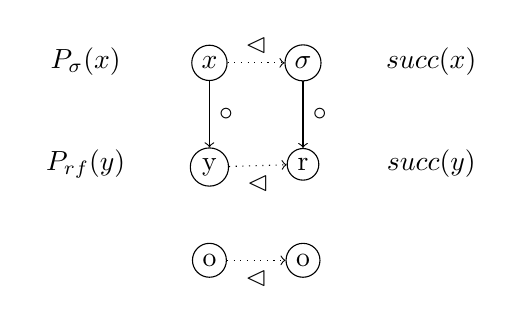
\begin{tikzpicture} [baseline = (m-1-1.base)]
\matrix (m) [matrix of nodes, column sep = 2em, row sep = 2em]{
$P_{\sigma}(x)$ & \node[draw,circle, inner sep =2pt](x1){$x$}; & \node[draw,circle, inner sep =2pt](x2){$\sigma$}; & $succ(x)$ \\
$P_{rf}(y)$ & \node[draw,circle, inner sep =2pt](y1){y}; & \node[draw,circle, inner sep =2pt](y2){r}; & $succ(y)$  \\
& \node[draw,circle, inner sep =2pt](z1){o}; & \node[draw,circle, inner sep =2pt](z2){o}; & \\
};
\draw [->] (x1) -- (y1) node[right, pos = .5]{$\circ$};
\draw [->] (x2) -- (y2) node[right, pos = .5]{$\circ$};
\draw [->, dotted] (x1) -- (x2) node[above, pos = .5]{$\vartriangleleft$};
\draw [->, dotted] (y1) -- (y2) node[below, pos = .5]{$\vartriangleleft$};
\draw [->, dotted] (z1) -- (z2) node[below, pos = .5]{$\vartriangleleft$};
\end{tikzpicture}
\end{center}
The availability of an order on the register nodes makes for cleaner definitions, but it is not as clearly motivated as syllable order and terminal node order. Assuming it for the time being, however, it is worth noting that it obviates the need to distinguish level and contour tones, since no reference to the terminal nodes is necessary. Using only syllable and t-node succession functions, an extra disjunct is needed in the case of contour tones, as in (\ref{Yipassw/cont}): 
\begin{equation} \label{Yipassw/cont}
\begin{aligned}
\alpha(x) = y \myeq P_{\sigma}(x)\,\land\,\delta(P_{cf}(y))\,\land\,\Big[&\big(\alpha(\delta(succ(y)))=succ(x)\big)\,\lor \\
&\big(\alpha(\delta(succ(succ(y))))=succ(x)\big)\Big]
\end{aligned} 
\end{equation} \par
We define dominance in a general Yip model in a similar way: a base case definition over unary relations (identical to the monosyllabic model under certain assumptions), with the inductive cases introducing successor relations. Much like the association function, definitions differ according to the degree of successor function specification. Unsurprisingly, imposing an order on the register nodes yields a simpler definition. Compare (\ref{yipd1}) and (\ref{yipd2}) below, where the former defines a successor function over register nodes while the latter does not.
\begin{align}
\delta(x)=y&\myeq P_{cf}(x)\land P_{rf}(y)\land[\delta(succ(x))=succ(y)] \label{yipd1} \\
\delta(x)=y&\myeq P_{cf}(x)\land \alpha(P_{\sigma}(y))\land[\alpha(succ(y))=\delta(succ(x))] \label{yipd2}
\end{align}  
Order on the register nodes creates a reference point for tones in succession, but this point is not crucial to defining the function.
\begin{center}
\begin{tikzpicture} [baseline = (m-1-1.base)]
\matrix (m) [matrix of nodes, column sep = 2em, row sep = 2em]{
& \node[draw,circle, inner sep =2pt](x1){o}; & \node[draw,circle, inner sep =2pt](x2){o}; &  \\
$P_{rf}(y)$ & \node[draw,circle, inner sep =2pt](y1){y}; & \node[draw,circle, inner sep =2pt](y2){r}; & $\delta(succ(x))$  \\
$P_{cf}(x)$& \node[draw,circle, inner sep =2pt](z1){x}; & \node[draw,circle, inner sep =2pt](z2){t}; & $succ(x)$ \\
};
\draw [->, dotted] (x1) -- (x2) node[above, pos = .5]{$\vartriangleleft$};
\draw [->, dotted] (y1) -- (y2) node[below, pos = .5]{$\vartriangleleft$};
\draw [->, dotted] (z1) -- (z2) node[below, pos = .5]{$\vartriangleleft$};
\draw [->] (z1) -- (y1) node[left, pos=.5]{$\delta$};
\draw [->] (z2) -- (y2) node[right, pos=.5]{$\delta$};
\end{tikzpicture}
\end{center}
Unlike the association definition, multiple disjuncts differentiate contour and level tones, even when the successor function is maximally-specified. The definition of dominance below reflects this. 
\begin{equation}
\begin{aligned}
\delta(x)=y\myeq P_{cf}\land P_{rf}(y)\land\Big[&\big(\delta(succ(x))=succ(y)\big)\lor \\
&\big(\delta(succ(succ(x)))=succ(y)\big)\Big]
\end{aligned}
\end{equation}
\begin{center}
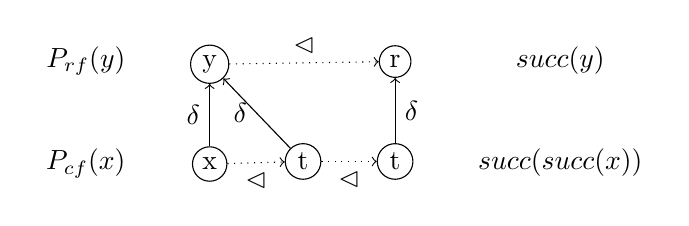
\begin{tikzpicture} [baseline = (m-1-1.base)]
\matrix (m) [matrix of nodes, column sep = 2em, row sep = 2em]{
$P_{rf}(y)$ & \node[draw,circle,inner sep=2pt](x1){y}; & & \node[draw,circle,inner sep=2pt](x2){r}; & $succ(y)$ \\
$P_{cf}(x)$ & \node[draw,circle,inner sep=2pt](y1){x}; & \node[draw,circle,inner sep=2pt](y2){t}; & \node[draw,circle,inner sep=2pt](y3){t}; & $succ(succ(x))$ \\
};
\draw[->, dotted] (x1) -- (x2) node[above, pos=.5]{$\vartriangleleft$};
\draw[->, dotted] (y1) -- (y2) node[below, pos=.5]{$\vartriangleleft$};
\draw[->, dotted] (y2) -- (y3) node[below, pos=.5]{$\vartriangleleft$};
\draw[->] (y1) -- (x1) node[left,pos=.5]{$\delta$};
\draw[->] (y2) -- (x1) node[left,pos=.5]{$\delta$};
\draw[->] (y3) -- (x2) node[right,pos=.5]{$\delta$};
\end{tikzpicture}
\end{center}
To summarize, association and dominance function definitions for the polysyllabic general Yip model are recursive, and utilize the successor function on specific tiers (our assumptions stipulate successor is defined for $\sigma, r, t$) to create reference points for multiple syllables.
\begin{equation}
\begin{aligned}
\alpha(x)=y&\myeq P_{\sigma}(x)\land P_{rf}(y)\land\big[\alpha(succ(x))=succ(y)\big] \\
\delta(x)=y&\myeq P_{cf}\land P_{rf}(y)\land\big[(\delta(succ(x))=succ(y))\lor(\delta(succ(succ(x)))=succ(y))\big]
\end{aligned}
\end{equation} \par
Extending Bao's model to polysyllabic forms follows in a similar fashion. Recall the model and the definition of association and dominance functions:
\begin{align}
\mathfrak{M}^{B} &\myeq \langle\mathfrak{D}; \mathcal{P}_{rf}, \mathcal{P}_{cf}, \mathcal{P}_{tbu}, P_{T}, P_{c}; \alpha(x), \delta(x), \mathtt{succ}(x)\rangle \\
\alpha(x)=y&\myeq \begin{cases} P_{T} & x=P_{\sigma} \end{cases} \\  
\delta(x)=y&\myeq \begin{cases} P_{T} & x\in\{P_{rf},P_{c}\} \\ P_{c} & x=P_{cf} \end{cases}
\end{align} 
By imposing an order on heterosyllabic tonal root (`T') nodes, the definition of the association function is similar to that of Yip's. The relationship is definable on level and contour tones equally.
\begin{equation} \label{Baoass}
\alpha(x)=y\myeq P_{\sigma}(x)\,\land\,P_{T}(y)\,\land\,[\alpha(succ(x))=succ(y)]
\end{equation}
Without this order, that is, with only an order on the terminal tonal nodes, a definition is possible, but is unsightly. In addition, a disjunction for level and contour tones is necessary, as reference is made to terminal tonal nodes.
\begin{equation}
\begin{aligned}
\alpha(x)=y\myeq P_{\sigma}(x)\land\delta(\delta(P_{cf}(y)))\Big[&\big(\alpha(\delta(\delta(succ(y))))=succ(x)\big)\,\lor \\
&\big(\alpha(\delta(\delta(succ(succ(y)))))=succ(x)\big)\Big]
\end{aligned}
\end{equation}
\begin{center}
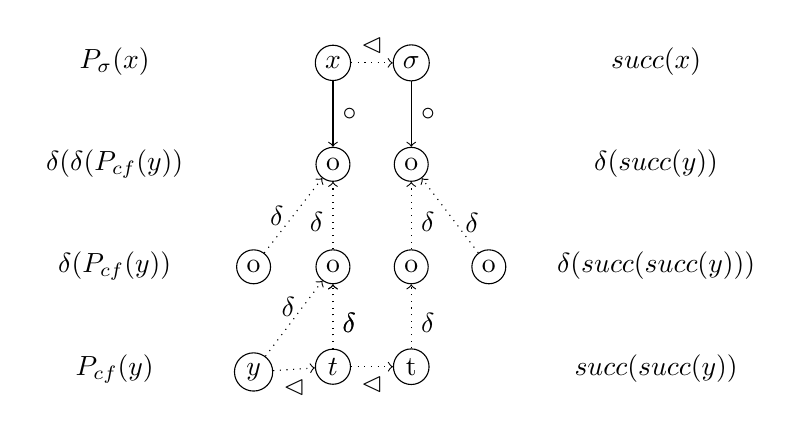
\begin{tikzpicture} [baseline = (m-1-1.base)]
\matrix (m) [matrix of nodes, column sep = 1.5em, row sep = 2em]{
$P_{\sigma}(x)$ & & \node[draw,circle, inner sep =2pt](x1){$x$}; & \node[draw,circle, inner sep =2pt](x2){$\sigma$}; & & $succ(x)$ \\
$\delta(\delta(P_{cf}(y))$ & & \node[draw,circle, inner sep =2pt](y1){o}; & \node[draw,circle, inner sep =2pt](y2){o}; & & $\delta(succ(y))$  \\
$\delta(P_{cf}(y))$ & \node[draw,circle, inner sep =2pt](j0){o}; & \node[draw,circle, inner sep =2pt](j1){o}; & \node[draw,circle, inner sep =2pt](j2){o}; & \node[draw,circle, inner sep =2pt](j3){o}; &  $\delta(succ(succ(y)))$  \\
$P_{cf}(y)$ & \node[draw,circle, inner sep =2pt](z0){$y$}; &  \node[draw,circle, inner sep =2pt](z1){$t$}; & \node[draw,circle, inner sep =2pt](z2){t};  & & $succ(succ(y))$ \\
};
\draw [->] (x1) -- (y1) node[right, pos = .5]{$\circ$};
\draw [->] (x2) -- (y2) node[right, pos = .5]{$\circ$};
\draw [->, dotted] (x1) -- (x2) node[above, pos = .5]{$\vartriangleleft$};
\draw [->, dotted] (z0) -- (z1) node[below, pos = .5]{$\vartriangleleft$};
\draw [->, dotted] (z1) -- (z2) node[below, pos = .5]{$\vartriangleleft$};
\draw [->, dotted] (z0) -- (j1) node[above, pos = .4]{$\delta$};
\draw [->, dotted] (z1) -- (j1) node[right, pos = .4]{$\delta$};
\draw [->, dotted] (z2) -- (j2) node[right, pos = .4]{$\delta$};
\draw [->, dotted] (j0) -- (y1) node[left, pos = .5]{$\delta$};
\draw [->, dotted] (j1) -- (y1) node[left, pos = .4]{$\delta$};
\draw [->, dotted] (z1) -- (j1) node[right, pos = .4]{$\delta$};
\draw [->, dotted] (j2) -- (y2) node[right, pos = .4]{$\delta$};
\draw [->, dotted] (j3) -- (y2) node[right, pos = .4]{$\delta$};
\end{tikzpicture}
\end{center} \par
The dominance function expands on the definition of association in (\ref{Baoass}), under the assumption that T, r, and c nodes are all ordered via $succ(x)$. Each instance (T dominates r, T dominates c, c dominates t) of domination forms a disjunct.
\begin{equation}
\begin{aligned}
\delta(x)=y\myeq\, &\Big[P_{rf}(x)\land P_{T}(y)\land[\delta(succ(x))=succ(y)]\Big]\,\lor \\
&\Big[P_{c}(x)\land P_{T}(y)\land[\delta(succ(x))=succ(y)]\Big]\,\lor \\
&\Big[P_{cf}(x)\land P_{c}(y)\land[\big(\delta(succ(x))=succ(y)\big)\lor\big(\delta(succ(succ(x)))=succ(y)\big)]\Big]
\end{aligned}
\end{equation}
The updated association and dominance functions in Bao's model are thus:
\begin{equation}
\begin{aligned}
\alpha(x)=y&\myeq P_{\sigma}(x)\,\land\,P_{T}(y)\,\land\,[\alpha(succ(x))=succ(y)] \\
\delta(x)=y&\myeq\, \Big[P_{rf}(x)\land P_{T}(y)\land[\delta(succ(x))=succ(y)]\Big]\,\lor \\
&\quad\,\,\,\Big[P_{c}(x)\land P_{T}(y)\land[\delta(succ(x))=succ(y)]\Big]\,\lor \\
&\quad\,\,\,\Big[P_{cf}(x)\land P_{c}(y)\land[\big(\delta(succ(x))=succ(y)\big)\lor\big(\delta(succ(succ(x)))=succ(y)\big)]\Big]
\end{aligned}
\end{equation}
Our assumptions have changed from the beginning of this writeup. Specifically, we have imposed orders via the succession function on all distinct elements in the models. Compare the figure below with the first figure, where we only assumed order on syllables and terminal nodes (domination and association are dotted).
\begin{center}
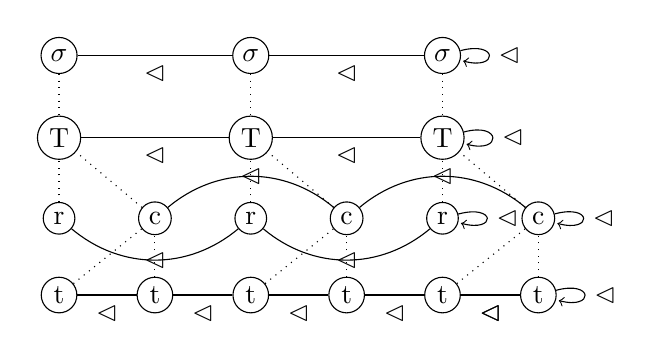
\begin{tikzpicture} [baseline = (x.base)]
\matrix (m) [matrix of nodes, column sep = 2em, row sep = 1.5em]{
\node[draw,circle, inner sep =2pt](x){$\sigma$}; & & \node[draw,circle, inner sep =2pt](x2){$\sigma$}; & & \node[draw,circle, inner sep =2pt](x3){$\sigma$};  \\
\node[draw,circle, inner sep =2pt](y){T}; & & \node[draw,circle, inner sep =2pt](y2){T}; & & \node[draw,circle, inner sep =2pt](y3){T};  \\
\node[draw,circle, inner sep =2pt](z){r}; & \node[draw,circle, inner sep =2pt](v){c}; & \node[draw,circle, inner sep =2pt](z2){r}; & \node[draw,circle, inner sep =2pt](v2){c}; & \node[draw,circle, inner sep =2pt](z3){r}; & \node[draw,circle, inner sep =2pt](v3){c};\\
\node[draw,circle, inner sep =2pt](q){t}; & \node[draw,circle, inner sep =2pt](s){t}; & \node[draw,circle, inner sep =2pt](q2){t}; & \node[draw,circle, inner sep =2pt](s2){t}; & \node[draw,circle, inner sep =2pt](q3){t}; & \node[draw,circle, inner sep =2pt](s3){t}; \\
};
\draw [dotted] (x) -- (y);
\draw [dotted] (z) -- (y);
\draw [dotted] (v) -- (y);
\draw [dotted] (q) -- (v);
\draw [dotted] (s) -- (v);
\draw (q) -- (s) node[below, pos=.5]{$\vartriangleleft$};
\draw [dotted] (x2) -- (y2);
\draw [dotted] (z2) -- (y2);
\draw [dotted] (v2) -- (y2);
\draw [dotted] (q2) -- (v2);
\draw [dotted] (s2) -- (v2);
\draw (q2) -- (s2) node[below, pos=.5]{$\vartriangleleft$};
\draw [dotted] (x3) -- (y3);
\draw [dotted] (z3) -- (y3);
\draw [dotted] (v3) -- (y3);
\draw [dotted] (q3) -- (v3);
\draw [dotted] (s3) -- (v3);
\draw (q3) -- (s3) node[below, pos=.5]{$\vartriangleleft$};
\draw (q3) -- (s3) node[below, pos=.5]{$\vartriangleleft$};
\draw (x) -- (x2) node[below, pos=.5]{$\vartriangleleft$};
\draw (x2) -- (x3) node[below, pos=.5]{$\vartriangleleft$};
\draw (s) -- (q2) node[below, pos=.5]{$\vartriangleleft$};
\draw (s2) -- (q3) node[below, pos=.5]{$\vartriangleleft$};
\path (x3) edge [loop right, align = center] node{$\vartriangleleft$} (x3);
\path (s3) edge [loop right, align = center] node{$\vartriangleleft$} (s3);
\draw (y) -- (y2) node[below, pos=.5]{$\vartriangleleft$};
\draw  (y2) -- (y3) node[below, pos=.5]{$\vartriangleleft$};
\path (y3) edge [loop right, align = center] node{$\vartriangleleft$} (y3);
\path (v) edge [bend left = 40] node{$\vartriangleleft$} (v2);
\path (v2) edge [bend left = 40] node{$\vartriangleleft$} (v3);
\path (v3) edge [loop right, align = center] node{$\vartriangleleft$} (v3);
\path (z) edge [bend right = 40] node{$\vartriangleleft$} (z2);
\path (z2) edge [bend right = 40] node{$\vartriangleleft$} (z3);
\path (z3) edge [loop right, align = center] node{$\vartriangleleft$} (z3);
\end{tikzpicture}
\hspace{1.2cm}
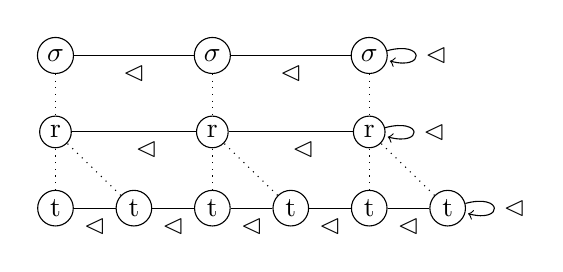
\begin{tikzpicture} [baseline = (x.base)]
\matrix (m) [matrix of nodes, column sep = 1.5em, row sep = 1.5em]{
\node[draw,circle, inner sep =2pt](x){$\sigma$}; & & \node[draw,circle, inner sep =2pt](x2){$\sigma$}; & & \node[draw,circle, inner sep =2pt](x3){$\sigma$};  \\
\node[draw,circle, inner sep =2pt](y){r}; & & \node[draw,circle, inner sep =2pt](y2){r}; & & \node[draw,circle, inner sep =2pt](y3){r};  \\
\node[draw,circle, inner sep =2pt](z){t}; & \node[draw,circle, inner sep =2pt](v){t}; & \node[draw,circle, inner sep =2pt](z2){t}; & \node[draw,circle, inner sep =2pt](v2){t}; & \node[draw,circle, inner sep =2pt](z3){t}; & \node[draw,circle, inner sep =2pt](v3){t};\\
};
\draw [dotted] (x) -- (y);
\draw [dotted] (z) -- (y);
\draw [dotted] (v) -- (y);
\draw [dotted] (x2) -- (y2);
\draw [dotted] (z2) -- (y2);
\draw [dotted] (v2) -- (y2);
\draw [dotted] (x3) -- (y3);
\draw [dotted] (z3) -- (y3);
\draw [dotted] (v3) -- (y3);
\draw (x) -- (x2) node[below, pos=.5]{$\vartriangleleft$};
\draw (x2) -- (x3) node[below, pos=.5]{$\vartriangleleft$};
\draw (v) -- (z2) node[below, pos=.5]{$\vartriangleleft$};
\draw (v2) -- (z3) node[below, pos=.5]{$\vartriangleleft$};
\draw (z) -- (v) node[below, pos=.5]{$\vartriangleleft$};
\draw (z2) -- (v2) node[below, pos=.5]{$\vartriangleleft$};
\draw (z3) -- (v3) node[below, pos=.5]{$\vartriangleleft$};
\path (x3) edge [loop right, align = center] node{$\vartriangleleft$} (x3);
\path (v3) edge [loop right, align = center] node{$\vartriangleleft$} (v3);
\draw (y) -- (y2) node[below, pos=.6]{$\vartriangleleft$};
\draw  (y2) -- (y3) node[below, pos=.6]{$\vartriangleleft$};
\path (y3) edge [loop right, align = center] node{$\vartriangleleft$} (y3);
\end{tikzpicture}
\end{center} \par
Two important questions remain. One is: are these extra orderings principled, or are they there just to simplify our definitions? I'm not sure. We have demonstrated that it is possible to derive definitions for dominance using only the ordering on syllable and terminal nodes, though the definitions themselves are a bit ugly. While these extra orderings may not be overtly motivated by the data, we have not included any that are explicitly unmotivated in the original theories, specifically an ordering on tautosyllabic register and `c' nodes. Bao claims that these nodes are unordered with respect to one another, such that the following structures are equivalent.
\begin{center}
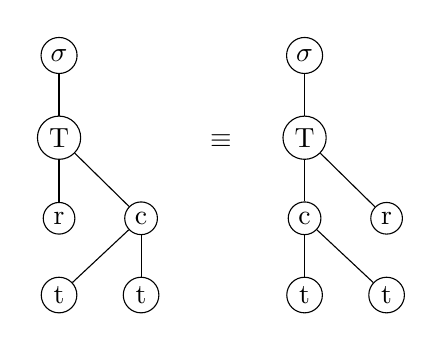
\begin{tikzpicture} [baseline = (x1.base)]
\matrix (m) [matrix of nodes, column sep = 1.5em, row sep = 1.5em]{
\node[draw,circle, inner sep =2pt](x1){$\sigma$}; & & & \node[draw,circle, inner sep =2pt](x2){$\sigma$};  \\
\node[draw,circle, inner sep =2pt](y1){T}; & & $\equiv$ & \node[draw,circle, inner sep =2pt](y2){T}; \\
\node[draw,circle, inner sep =2pt](z1){r}; & \node[draw,circle, inner sep =2pt](z2){c}; & & \node[draw,circle, inner sep =2pt](z3){c}; & \node[draw,circle, inner sep =2pt](z4){r}; \\
\node[draw,circle, inner sep =2pt](t1){t}; & \node[draw,circle, inner sep =2pt](t2){t}; & & \node[draw,circle, inner sep =2pt](t3){t}; & \node[draw,circle, inner sep =2pt](t4){t}; \\
};
\draw (x1) -- (y1);
\draw (x2) -- (y2);
\draw (z1) -- (y1);
\draw (z2) -- (y1);
\draw (z2) -- (t1);
\draw (z2) -- (t2);
\draw (y2) -- (z3);
\draw (y2) -- (z4);
\draw (z3) -- (t3);
\draw (z3) -- (t4);
\end{tikzpicture}
\end{center}
Another question concerns the definition of $succ(x)$; it forms a crucial part of our definitions of association and dominance, but it does not itself have an explicit definition. Again, I'm not exactly sure how to do this, but the intuition is that successor is a total function on all nodes of each tier. That is, it is defined over syllable nodes, T nodes, register nodes, c nodes, and terminal nodes separately, but not between them. There are a number of approaches to ensuring this. One is to have a different successor function for each type. Another is to define successor as a unary function (viz Chandlee and Lindell (2016)) with multiple disjuncts that limit it to a particular type via the unary relations. Note again that the final position is also its own successor.
\begin{equation}
succ(x) = (P_{\sigma}(x)\land x+1) \lor(P_{rf}(x)\land x+1) ...
\end{equation}
Since it's a unary function, I don't know whether this definition will guarantee that the order only holds within a set of elements which share the same label. I need to work on this more.
\end{document}